\chapter{Results}
\lhead{\chaptername~\thechapter. \emph{Spherical SfM}}
In this chapter, we comment the results obtained with our SfM pipeline.
We tested our approach with both some computer-generated and real environments.
We compare the pose estimation results with ground truth in the synthetic cases
while we only give a qualitative evaluation for the multi-view stereo
reconstruction step for both the synthetic and real video sequences.
We obtained all the results with MATLAB R2017a on a \todo{aggiungere caratteristiche macchina laboratorio}

\section{Data Sets Description}
\subsection{Synthetic Scenes}
The first synthetic environment is a simple one we created in Blender 2.78c;
it is composed of a room with 5 polyhedrons. We added some image textures to both
the room's walls and the shapes' faces to reduce matching outliers.
The camera moves in a continuous curve around the polyhedrons and both its
position and orientation change.
Figure~\ref{fig:test6} shows some rendered images for this environment.
%
\begin{figure}
\centering
	\begin{subfigure}{0.4\textwidth}
		\centering
		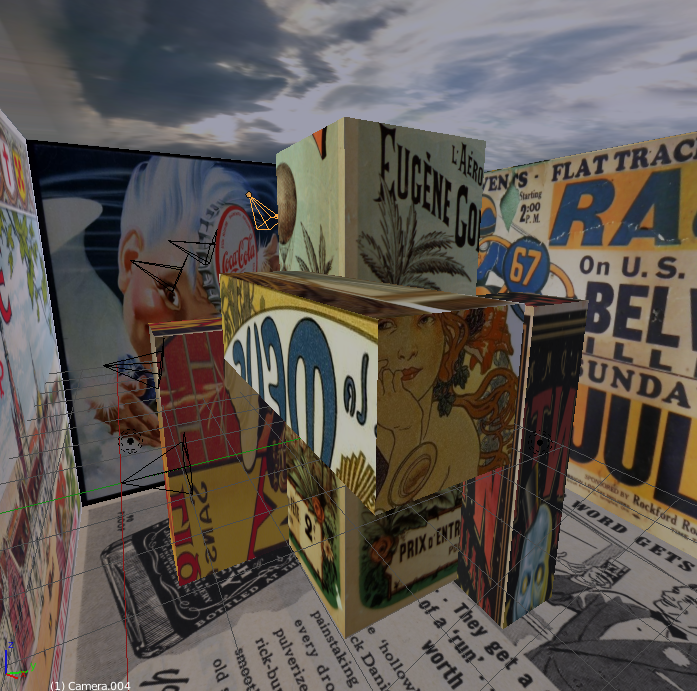
\includegraphics[width=\textwidth]{img/test6_1}
	\end{subfigure}
    %
	\begin{subfigure}{0.4\textwidth}
		\centering
		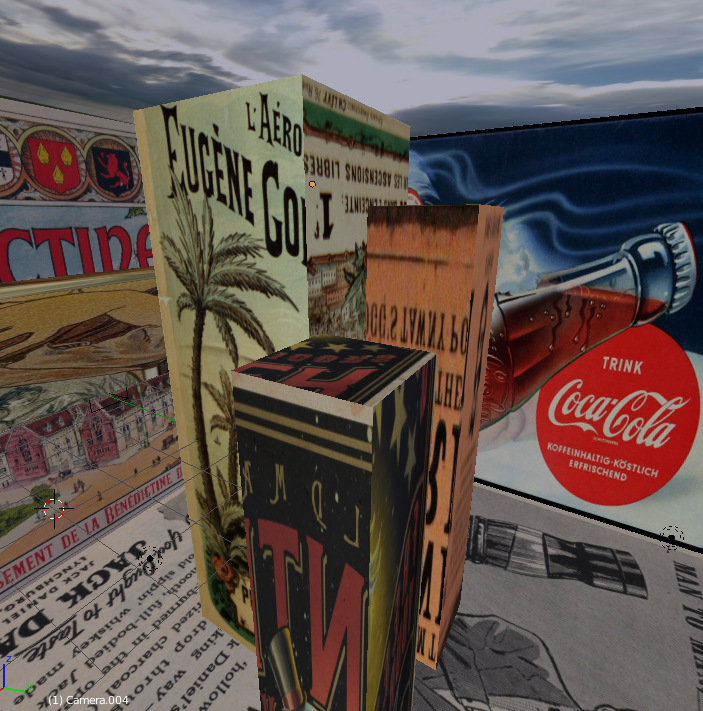
\includegraphics[width=\textwidth]{img/test6_2}
	\end{subfigure}
    %
	\begin{subfigure}{0.4\textwidth}
		\centering
		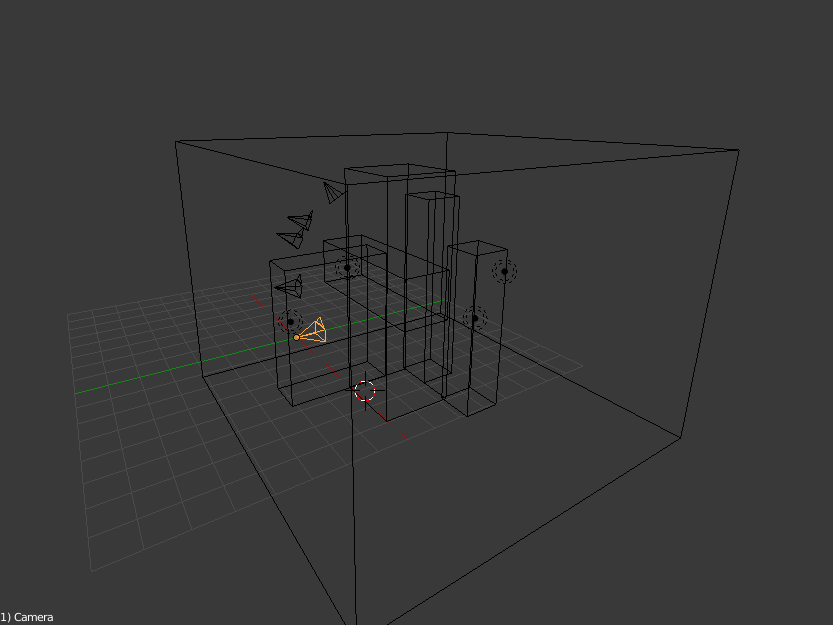
\includegraphics[width=\textwidth]{img/test6_3}
	\end{subfigure}
    %
	\begin{subfigure}{0.4\textwidth}
		\centering
		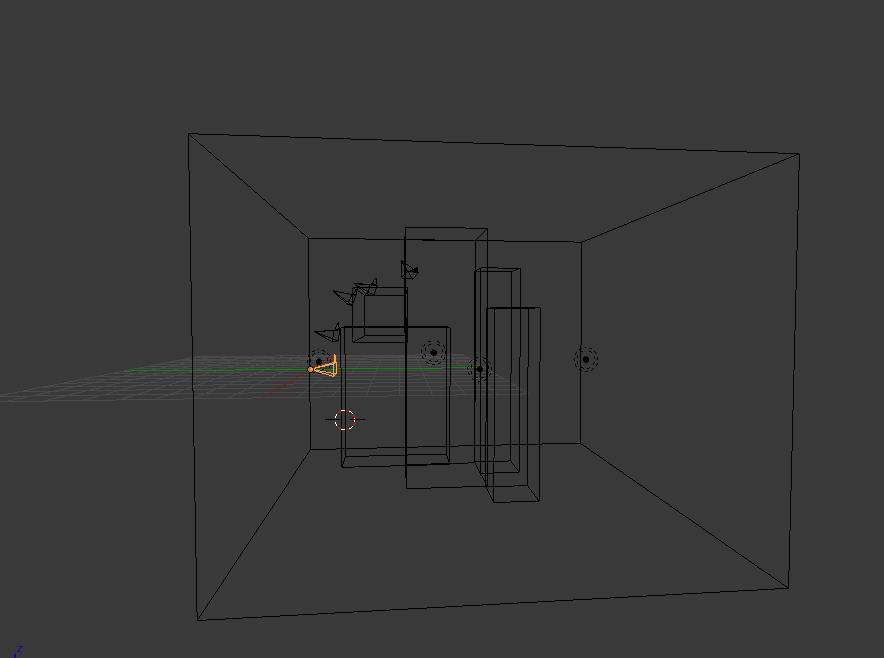
\includegraphics[width=\textwidth]{img/test6_4}
	\end{subfigure}
	%
	\begin{subfigure}{0.8\textwidth}
		\centering
		\includegraphics[width=\textwidth]{img/test6_5}
	\end{subfigure}
	%
	\caption{The first computer-generated environment we use in our test and
	an example equirectangular image from this scene: two views of the scene (top row),
	wireframe visualizations of the same scene (middle row), and an example
	equirectangular image produced with this set up (bottom row).}
    \label{fig:test6}
\end{figure}
%

In the second synthetic scene, we recreated a town square surrounded by
a covered walk (loggia). The roof of the walk is supported by columns on the inner
side, the one that is oriented toward the square's centre, and by a wall on the
outer side.
Again the environment is contained in a room and every surface is textured.
The camera moves along the walk with a non-uniform speed while pointing toward
the centre of the square. Figure~\ref{fig:test_square} shows some images
for this second environment.
%
\begin{figure}
\centering
	\begin{subfigure}{0.4\textwidth}
		\centering
		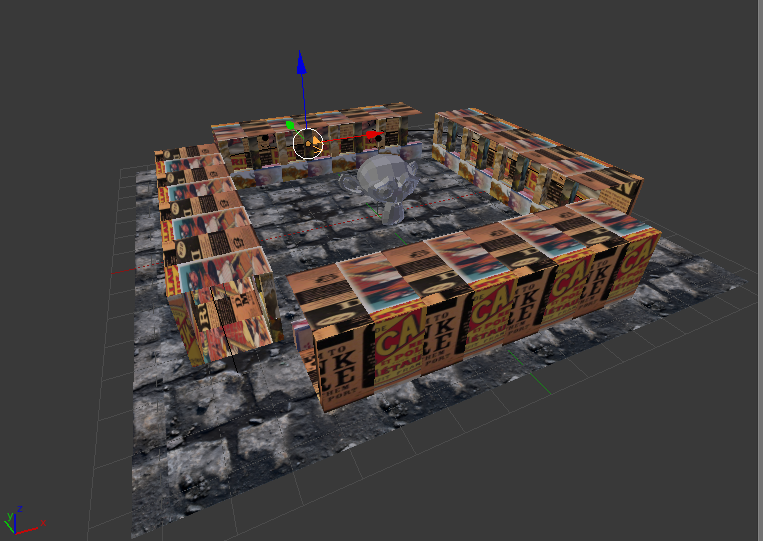
\includegraphics[width=\textwidth]{img/square1}
	\end{subfigure}
    %
	\begin{subfigure}{0.4\textwidth}
		\centering
		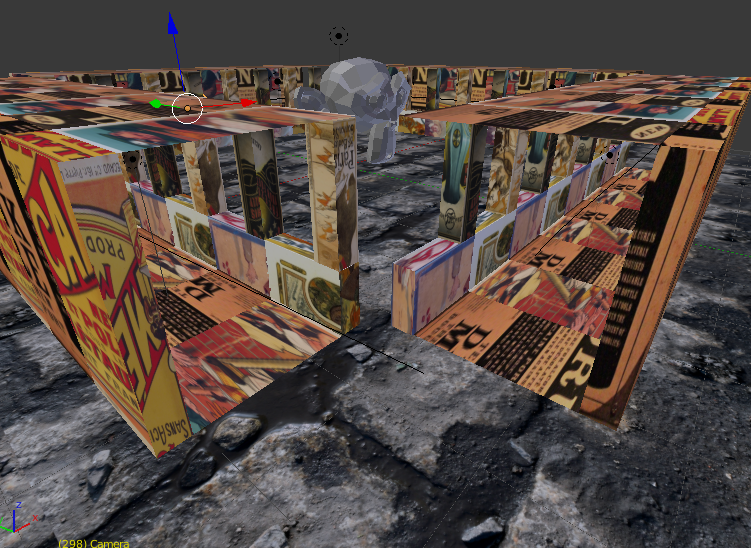
\includegraphics[width=\textwidth]{img/square2}
	\end{subfigure}
    %
	\begin{subfigure}{0.8\textwidth}
		\centering
		\includegraphics[width=\textwidth]{img/square3}
	\end{subfigure}
    %
	\begin{subfigure}{0.8\textwidth}
		\centering
		\includegraphics[width=\textwidth]{img/square4}
	\end{subfigure}
	%
	\caption{The computer-generated town square environment: two views of the
	model (top row) and a two example equirectangular images produced from this
	scene (middle and bottom row).}
    \label{fig:test_square}
\end{figure}

\subsection{Real environment}\label{subsec:real_environment}
We test our pipeline with a real video footage too. We do not have the ground truth
for the camera poses in the real environment but the quality of the
reconstruction is an indicator of the pipeline performance.
We captured the real sequence with the Ricoh Theta S camera in a town square
surrounded by a loggia. Again we walked around the square, along the covered
walks, keeping the camera above the user's head thanks to a stick.
The user does not influence the camera poses estimation since it appears in the
pole region of the image sphere and, as we said in
Section~\ref{sec:pipeline_pose_estimation}, we discard potential matches in
these areas.
We present some pictures of the real environment together with some examples
of the equirectangular images of the town square in
Figure~\ref{fig:piazzaLeoni}.
%
\begin{figure}[h]
\centering
	\begin{subfigure}{0.7\linewidth}
		\centering
		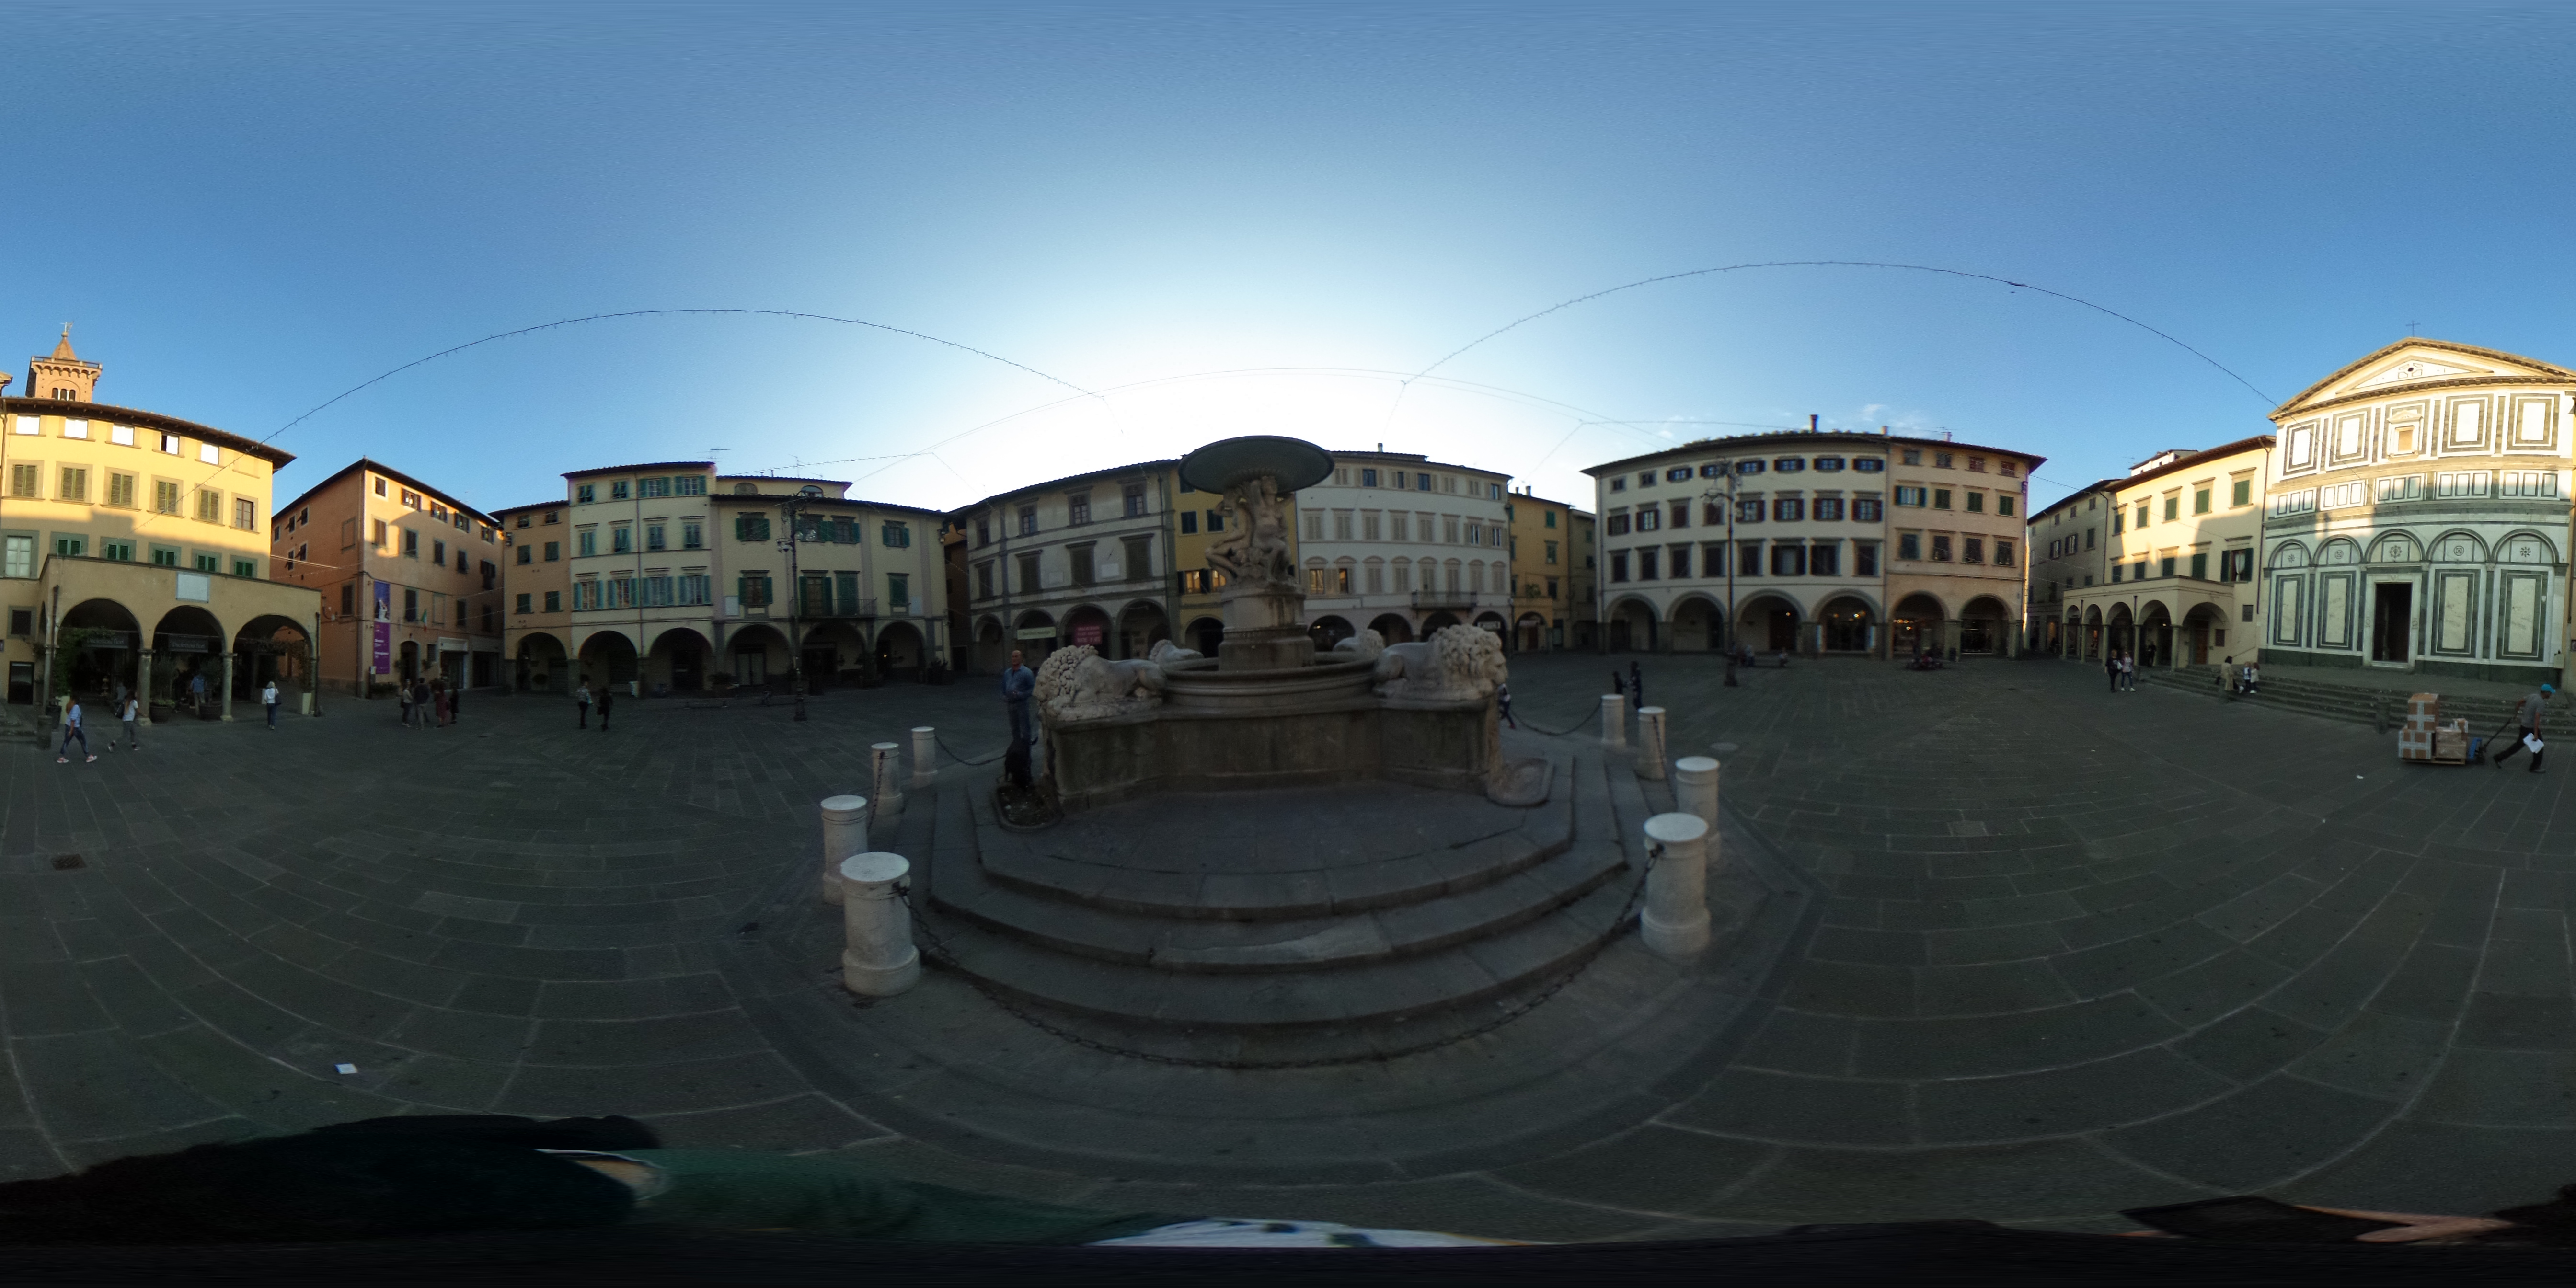
\includegraphics[width=\linewidth]{img/piazzaLeoni.jpg}
		\caption{Panoramic view of the real town square.}
	\end{subfigure}
	%
	\begin{subfigure}{0.7\linewidth}
		\centering
		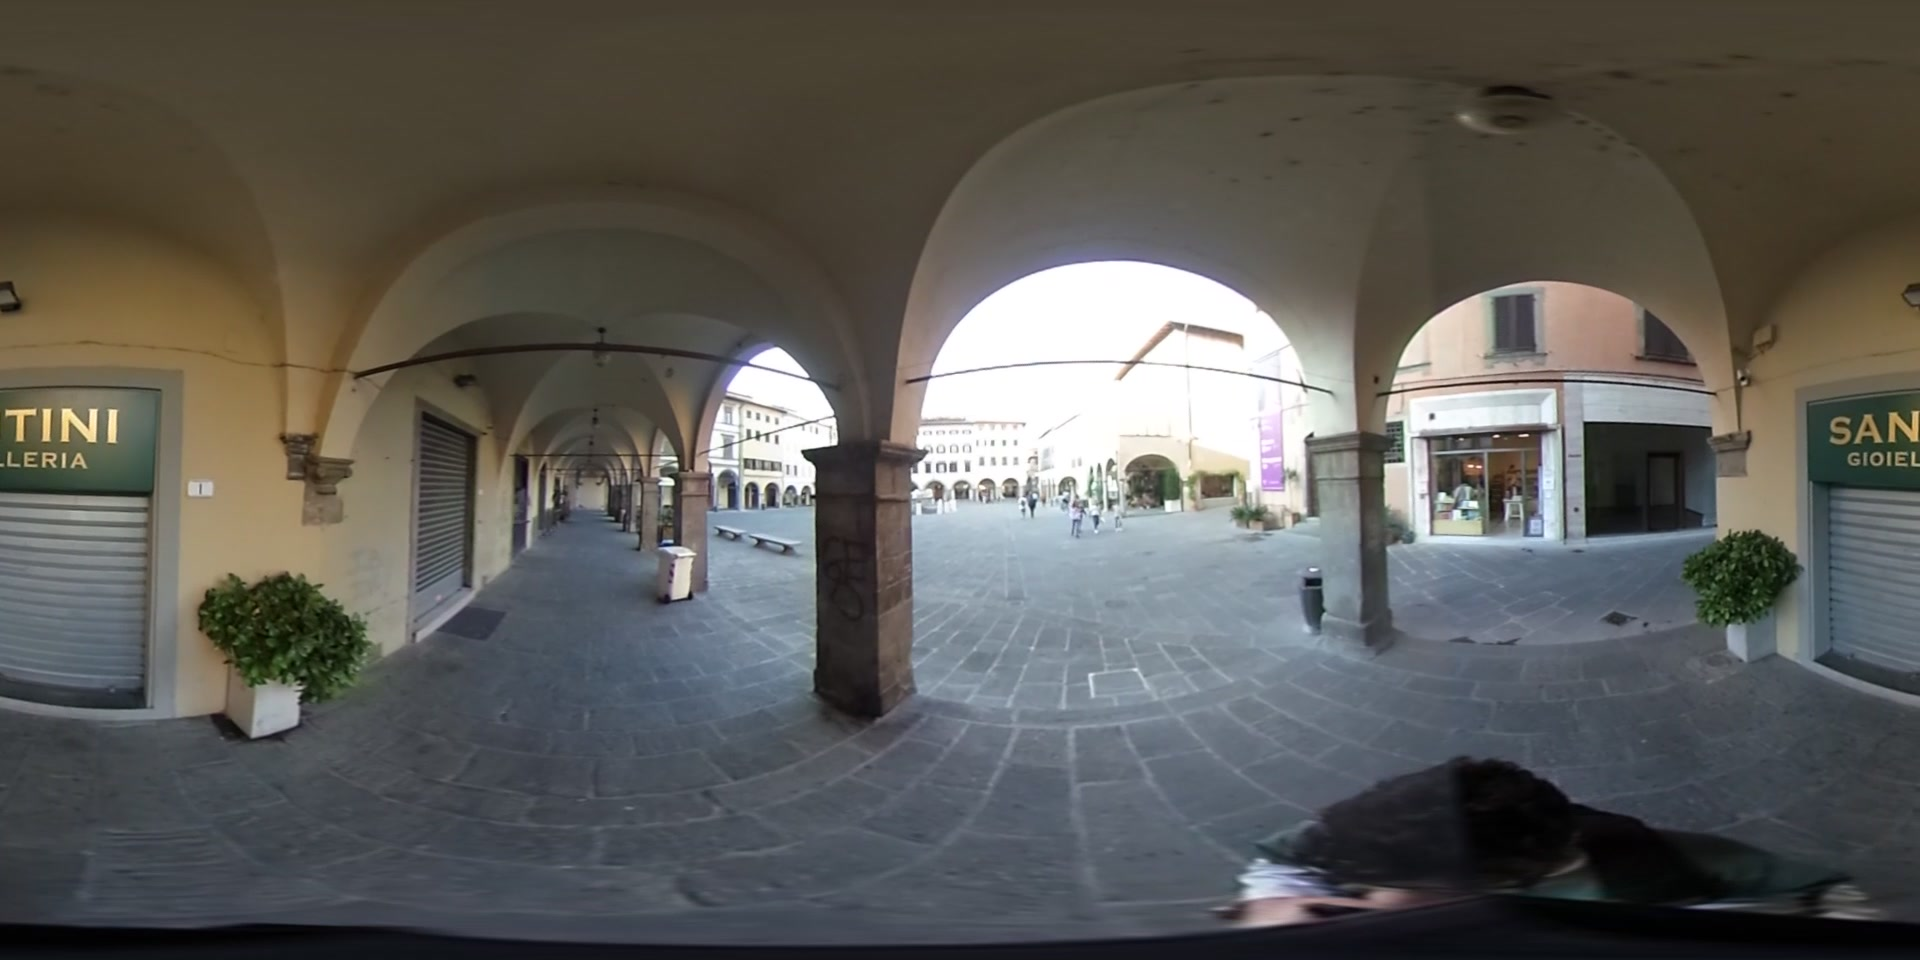
\includegraphics[width=\linewidth]{img/piazzaLeoni_exampleds.jpg}
		\caption{Example frame from the real town square sequence.}
	\end{subfigure}
\caption{The town square we use in our real reconstruction test.}
\label{fig:piazzaLeoni}
\end{figure}

\section{Experiment Results}
\subsection{Window Size Test}
We perform an experiment to chose the optimal window size for the windowed
bundle adjustment (Section~\ref{subsec:windowed_ba}). In this experiment we
use the synthetic town square and compute the sum of absolute pose error, in
particular, we find the location and orientation errors for the estimated poses.
Figure~\ref{fig:sumAbsLocError} shows the comparison of the resulted location error for 20
estimated poses with respect to several windowed and non-windowed adjustment
techniques.
In particular, we can see that the pose error is minimal when we employ the
windowed bundle adjustment with a window that contains 5 poses at a time.
Windows smaller than 5 do not bring substantial improvements (remember that,
as we pointed out in Section~\ref{subsec:windowed_ba}, to maintain the proper scale, we keep the two poses
in a window fixed), while the error also increases
for larger windows. The performance deterioration when using larger windows
is due to the fact that the windowed adjustment may suffer from the high number
of views to be optimized: if a series of views with wrong estimated poses are
already inside the window and a new pose enters it, the prevalent number of
bad estimation may result in the last pose to be aligned to the wrong trajectory
of the previous estimations. Because of this phenomenon, all the next views
may be incorrectly optimized, thus reducing the performance of the overall
pose estimation.
%
\begin{figure}[h]
\centering
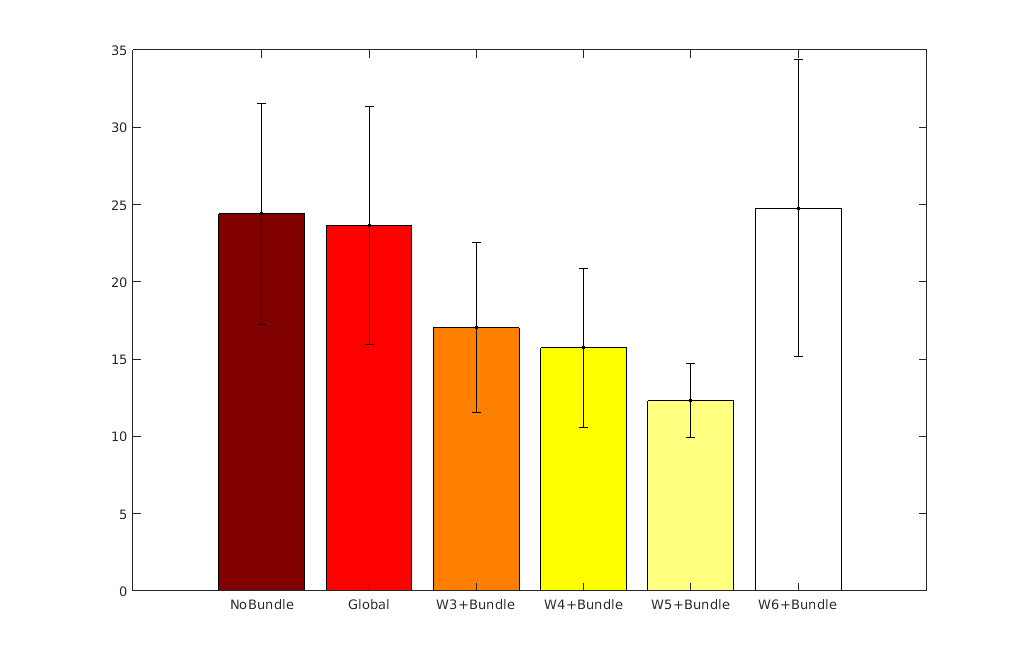
\includegraphics[width=\linewidth]{img/sumAbsLocError.png}
\caption{How the location error varies with respect to the adjustment technique
used. Angular errors present a similar behaviour with a minimum in case
of windowed bundle adjustment whose window length set to 5 views.}
\label{fig:sumAbsLocError}
\end{figure}

\subsection{Essential Matrix Estimation Test}\label{subsec:essential_test}
In Section~\ref{subsec:essential_estimation} we said that our pipeline
calls the essential matrix estimation routine until the fraction of inliers
drops below a threshold. In Figure~\ref{fig:essential_test} we show the
results of an experiment where we compare three different essential matrix
evaluation approaches. The input data for this experiment is composed of
a set of manually selected frames from the first synthetic environment.
The reason why we select the frames is that we do not want this results to be
influenced by the frame filter.
%
\begin{figure}[h]
\centering
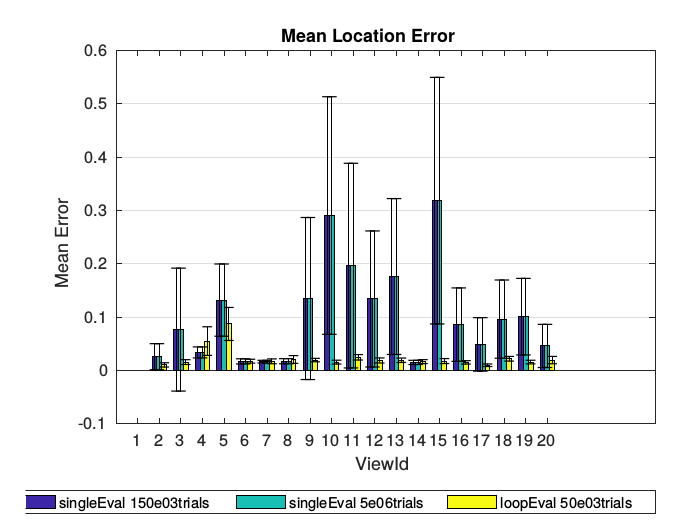
\includegraphics[width=\linewidth]{img/essentialEstimation.png}
\caption{How the location error changes with respect to different essential
matrix estimation function approaches: the purple and light blue columns
represent the average location error results for each frame when the
essential estimation is performed with a single call to the routine, while the
yellow column represent the location error when we perform the estimation
again when the fraction of inliers is too low.}
\label{fig:essential_test}
\end{figure}

\subsection{SfM Phase Result}
In this test, we analysed the overall results of the initial step of our
pipeline, the motion estimation phase. We use the 365 rendered frame of our
synthetic town square environment. Figure~\ref{fig:trajectory} shows the actual
and estimated trajectory of the camera in the synthetic environment.
%
\todo[inline]{Devo ancora cambiare l'immagine\ref{fig:trajectory} aggiungendo i punti sparsi 
ottenuti da sfm e eventualmente scegliere un tratto piu' interessante in cui la camera fa una curva.}
%
\begin{figure}[h]
\centering
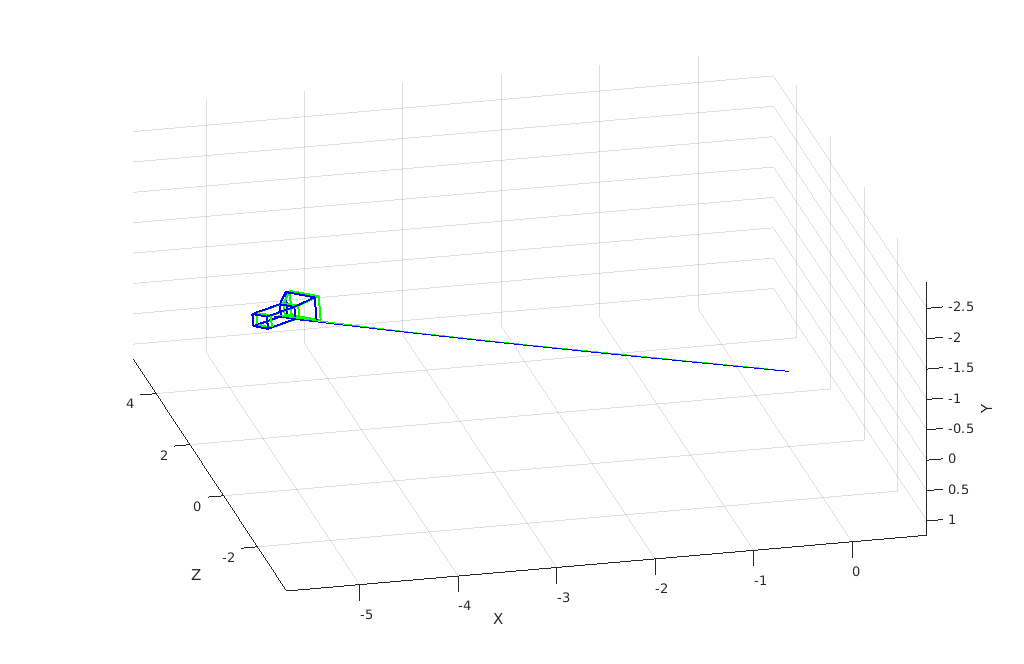
\includegraphics[width=\linewidth]{img/trajectory.png}
\caption{The comparison between the estimated trajectory (blue line) and
actual trajectory (green line). as we can see the pose estimation is very close
to the actual path.}
\label{fig:trajectory}
\end{figure}
%
\subsection{Disparity Maps}
Figure~\ref{fig:llDisparity} shows an example of disparity map computed
with our adaptive block-matching algorithm. Darker colours refer to the points
with less disparity thus, farther from the camera. On the other hand, the closer
objects have brighter colours.
%
\begin{figure}[h]
\centering
	\begin{subfigure}{0.7\linewidth}
		\centering
		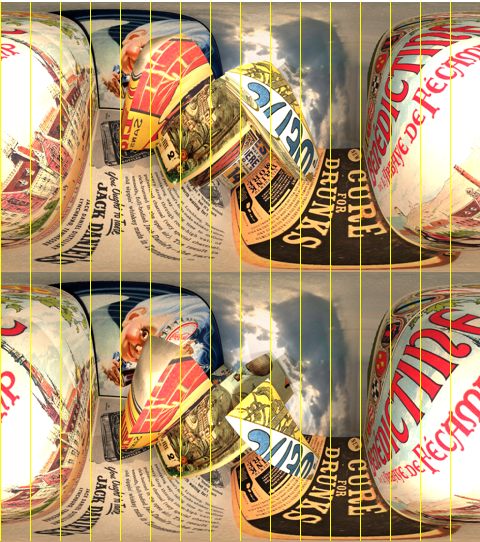
\includegraphics[width=\linewidth]{img/rectified_pair.png}
		\caption{Original rectified pair.}
	\end{subfigure}
	%
	\begin{subfigure}{0.7\linewidth}
		\centering
		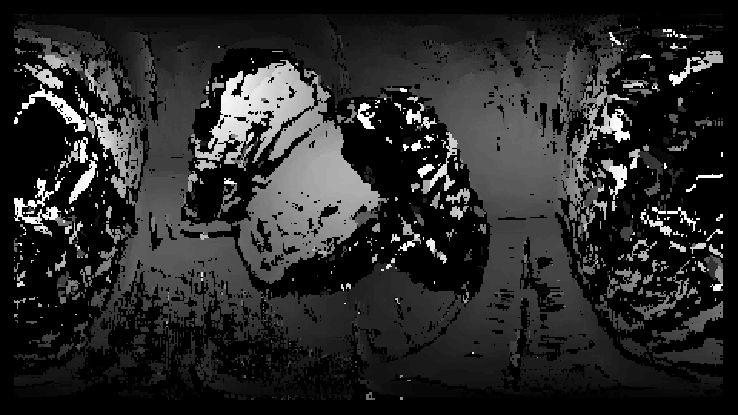
\includegraphics[width=\linewidth]{img/lldisparity2.png}
		\caption{Computed disparity map.}
	\end{subfigure}
\caption{An example of disparity map computed with our adaptive block-matching
algorithm. The black point in the map are points whose disparity is equal to
zero or that are occluded in the other image; in both cases, these points are
not triangulated.}
\label{fig:llDisparity}
\end{figure}

\subsection{Environments Reconstruction}
Figure~\ref{fig:real_reconstruction} shows the resulting reconstruction of the
real town square's loggia described in Section~\ref{subsec:real_environment}.
%
\todo[inline]{Questa ricostruzione e' solo una prova limitata a 4 coppie di view.}
\begin{figure}[h]
\centering
	\begin{subfigure}{0.45\linewidth}
		\centering
		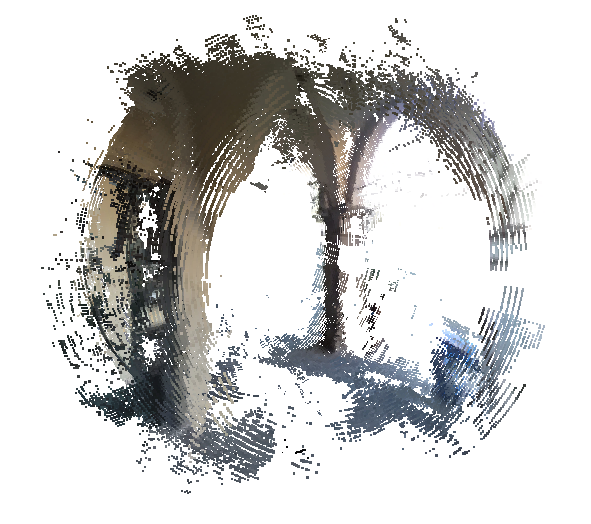
\includegraphics[width=\linewidth]{img/reconstruction1.png}
	\end{subfigure}
	%
	\begin{subfigure}{0.45\linewidth}
		\centering
		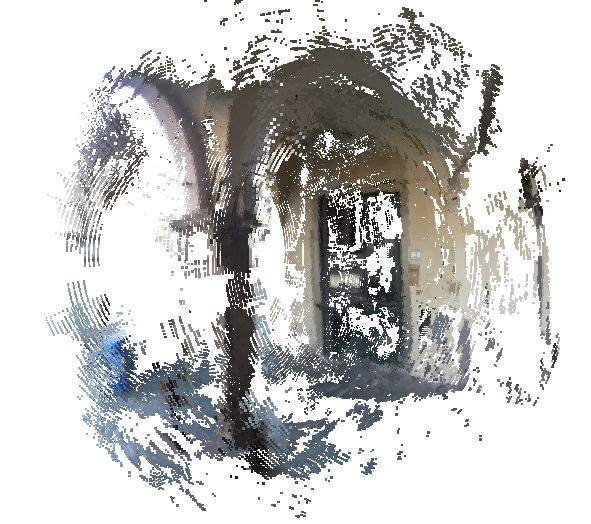
\includegraphics[width=\linewidth]{img/reconstruction2.png}
	\end{subfigure}
	\caption{Two views of the dense point cloud of the real town square
	(Section~\ref{subsec:real_environment}) obtained with our SfM pipeline.}
	\label{fig:real_reconstruction}
\end{figure}
